\documentclass{article}
\usepackage{pgfplots}
\pgfplotsset{compat=1.7}

\begin{document}


\begin{figure}[!t]
\centering
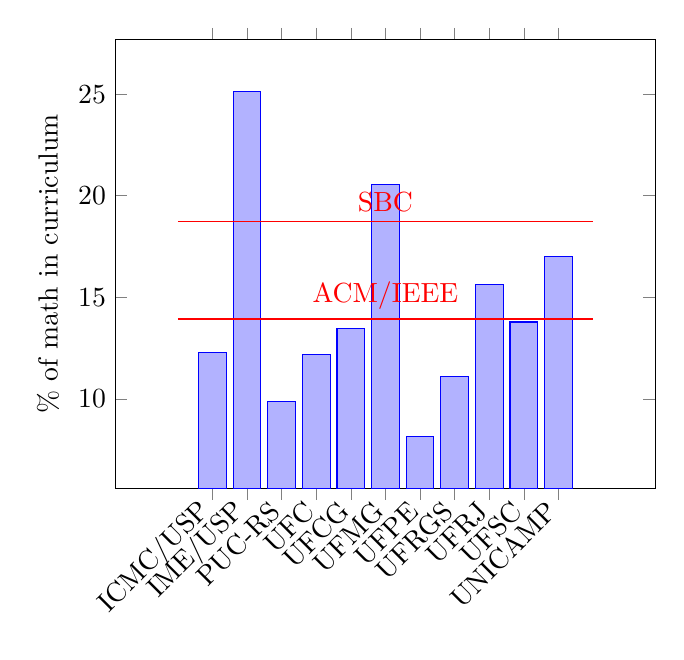
\begin{tikzpicture}
	\begin{axis}[
	ybar,
	enlargelimits=0.15,
	legend style={at={(0.5,-0.15)},
	anchor=north,legend columns=-1},
	ylabel={\% of math in curriculum},
	symbolic x coords={pre,ICMC/USP,IME/USP,PUC-RS,UFC,UFCG,UFMG,UFPE,UFRGS,UFRJ,UFSC,UNICAMP,pos},
	xtick=data,
%	nodes near coords,
%	nodes near coords align={vertical},
	x tick label style={rotate=45,anchor=east},
	]
	
	\addplot 
		coordinates {(ICMC/USP,12.29) (IME/USP,25.13) (PUC-RS,9.85) (UFC,12.20) (UFCG,13.46) (UFMG,20.57) (UFPE,8.15) (UFRGS,11.11) (UFRJ,15.61) (UFSC,13.78) (UNICAMP,17.00)};
	\addplot[red,sharp plot]
		coordinates {(pre,13.93) (pos,13.93)}
		node[above] at (axis cs:UFMG,13.93) {ACM/IEEE};
	\addplot[red,sharp plot]
		coordinates {(pre,18.75) (pos,18.75)}
		node[above] at (axis cs:UFMG,18.75) {SBC};
\end{axis}
\end{tikzpicture}
\caption{The proportion of mathematics in each curriculum compared with the reference curricula}
\end{figure}

\end{document}
